% Adjust these for the path of the theme and its graphics, relative to this file
%\usepackage{beamerthemeFalmouthGamesAcademy}
\usepackage{../../beamerthemeFalmouthGamesAcademy}
\usepackage{multimedia}
\graphicspath{ {../../} }

% Default language for code listings
\lstset{language=C++,
        morekeywords={each,in,nullptr}
}

% For strikethrough effect
\usepackage[normalem]{ulem}
\usepackage{wasysym}

\usepackage{pdfpages}

% http://www.texample.net/tikz/examples/state-machine/
\usetikzlibrary{arrows,automata}

\newcommand{\modulecode}{COMP702}\newcommand{\moduletitle}{Classical Artificial Intelligence}\newcommand{\sessionnumber}{1}

\hypersetup{
pdftex,
pdftitle=\sessionnumber: Navigation,
pdfauthor=Ed Powley,
pdfdisplaydoctitle,
pdflang=en-GB
}

\begin{document}
\title{\sessionnumber: Navigation}
\subtitle{\modulecode: \moduletitle}

\frame{\titlepage} 

\begin{frame}{Paper Club}
	For next week's session:
	
	Nathan R.\ Sturtevant, Devon Sigurdson, Bjorn Taylor, Tim Gibson.
	Pathfinding and Abstraction with Dynamic Terrain Costs.
	Proceedings of AIIDE Conference, 2019.
	
	(PDF link on LearningSpace)
\end{frame}

\part{Pathfinding}
\frame{\partpage}

\begin{frame}{The problem}
    \begin{itemize}
        \item We have a \textbf{graph} \pause
            \begin{itemize}
                \item \textbf{Nodes} (points) \pause
                \item \textbf{Edges} (lines between points, each with a \textbf{length}) \pause
            \end{itemize}
        \item E.g.\ a road map \pause
            \begin{itemize}
                \item Nodes = addresses \pause
                \item Edges = roads \pause
            \end{itemize}
        \item E.g.\ a tile-based 2D game \pause
            \begin{itemize}
                \item Nodes = grid squares \pause
                \item Edges = connections between adjacent squares \pause
            \end{itemize}
        \item Given two nodes $A$ and $B$, find the \textbf{shortest path} from $A$ to $B$ \pause
            \begin{itemize}
                \item ``Shortest'' in terms of edge lengths --- could be distance, time, fuel cost, ...
            \end{itemize}
    \end{itemize}
\end{frame}

\begin{frame}{Applications of pathfinding}
    \begin{center}
        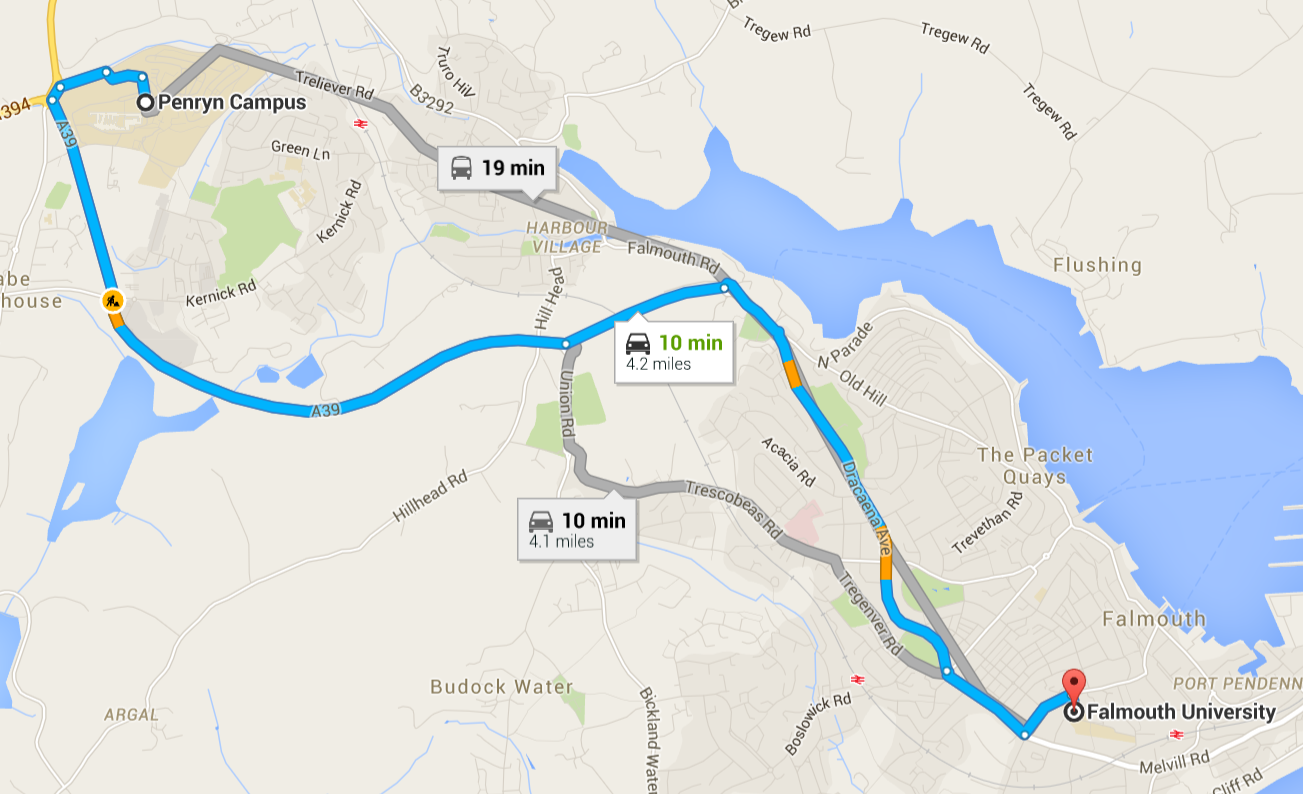
\includegraphics[width=\textwidth]{pathfinding_1}
    \end{center}
\end{frame}

\begin{frame}{Applications of pathfinding}
    \begin{center}
        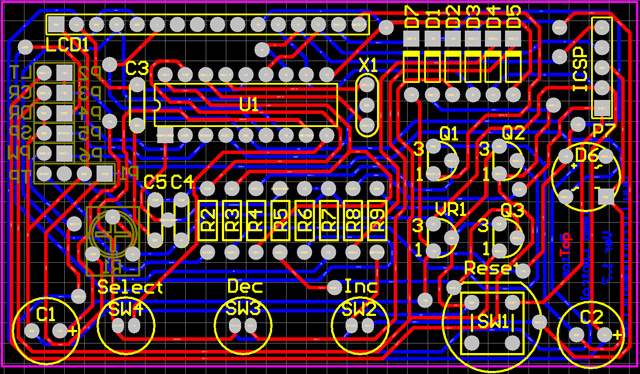
\includegraphics[width=\textwidth]{pcb}
    \end{center}
\end{frame}

\begin{frame}{Applications of pathfinding}
    \begin{center}
        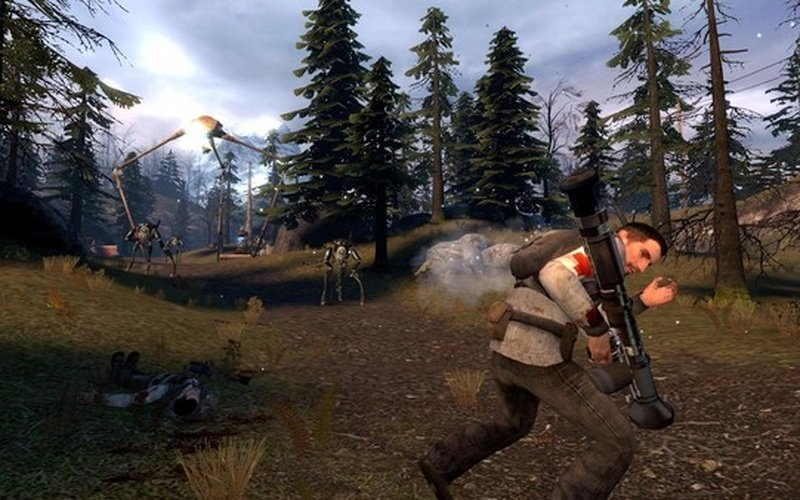
\includegraphics[width=\textwidth]{image5}
    \end{center}
\end{frame}

\begin{frame}{Applications of pathfinding}
    \begin{center}
        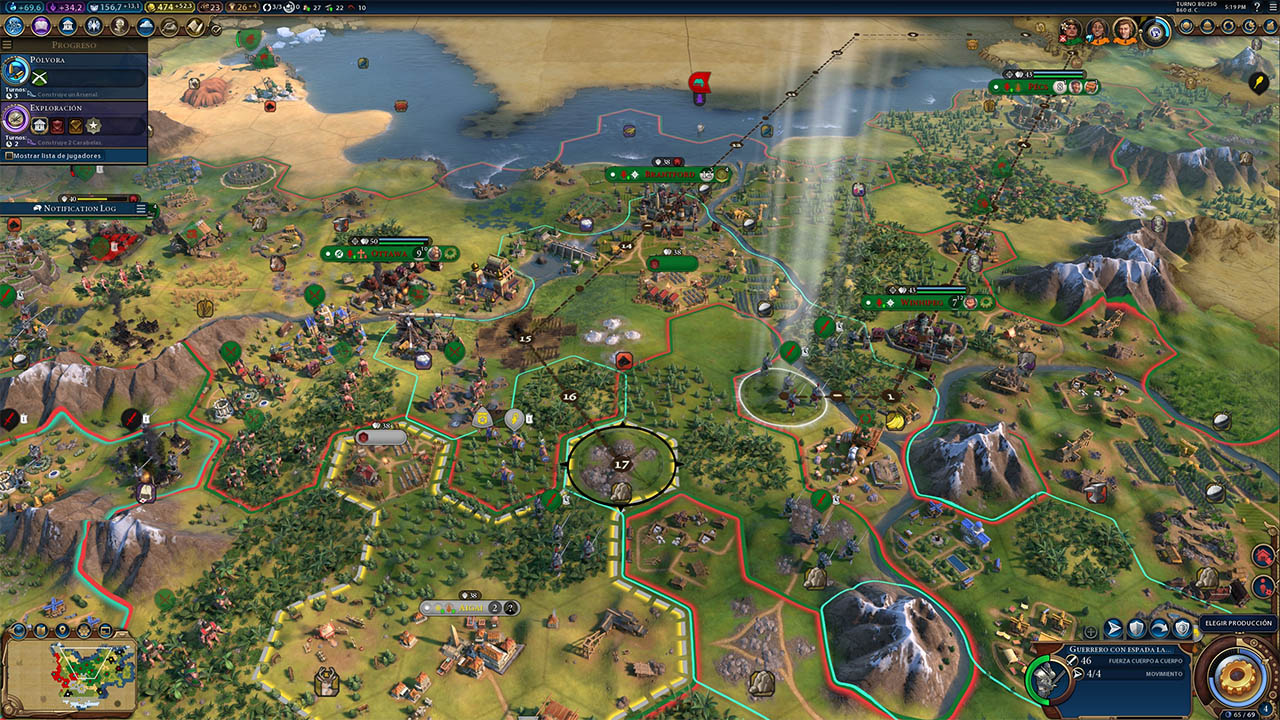
\includegraphics[width=\textwidth]{image6}
    \end{center}
\end{frame}

\begin{frame}{Applications of pathfinding}
    \begin{center}
        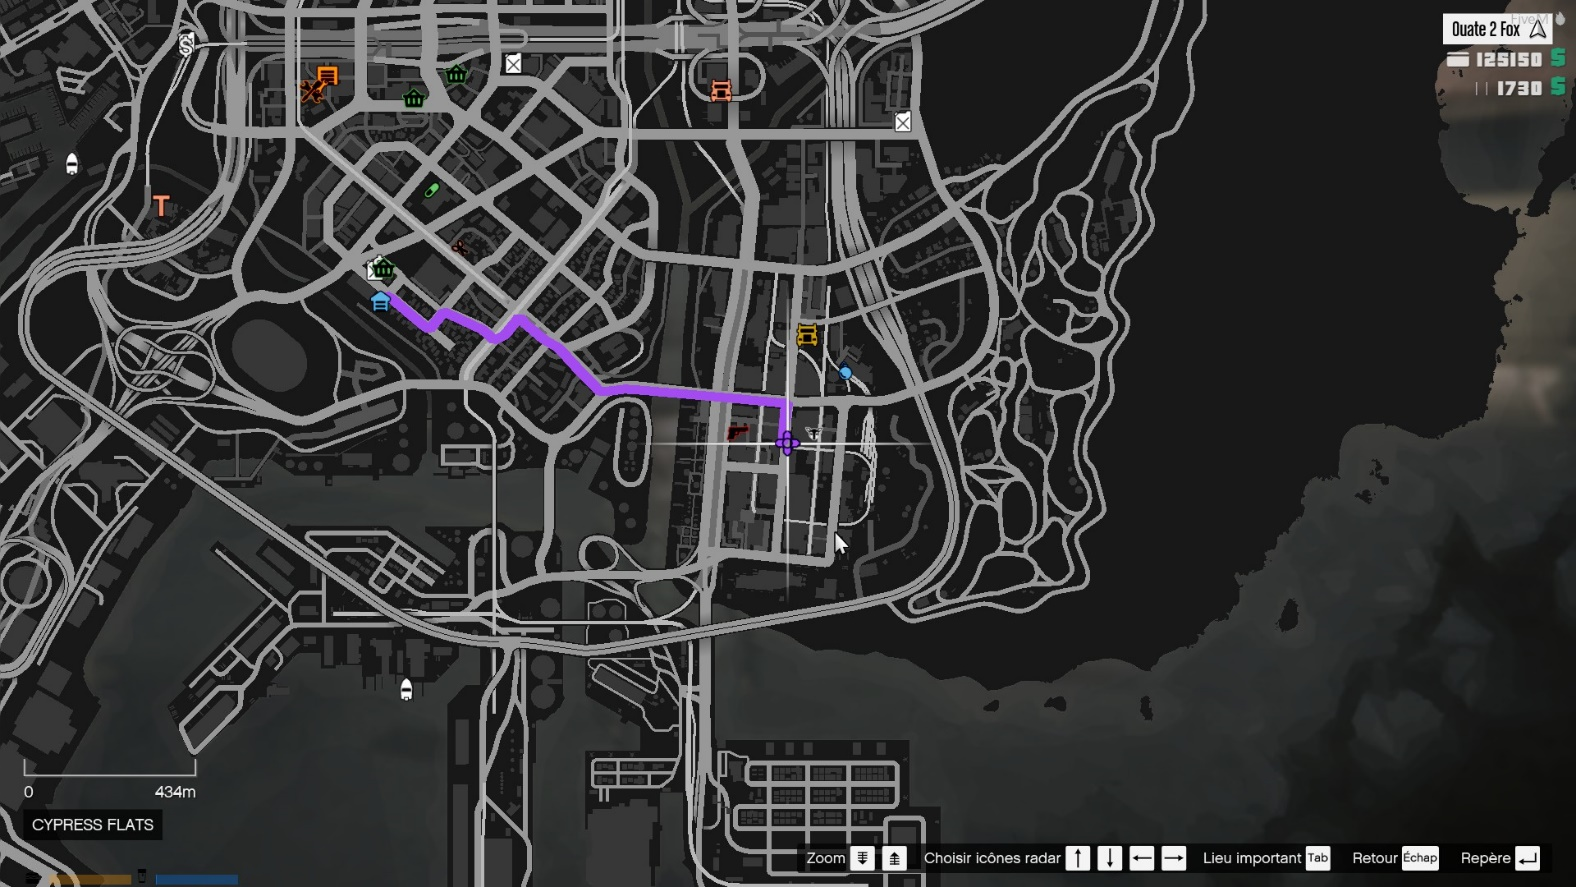
\includegraphics[width=\textwidth]{image7}
    \end{center}
\end{frame}

\begin{frame}{Pathfinding as search}
    \begin{itemize}
        \pause\item Basic idea: build a \textbf{spanning tree} for the graph
        \pause\item Root node is $A$ (the start node)
        \pause\item Edges in the tree are a \textbf{subset} of edges of the graph
        \pause\item Once the tree includes $B$, we can read off the path from $A$ to $B$
        \pause\item Need to keep track of two sets of nodes:
            \begin{itemize}
                \pause\item \textbf{Open set}: nodes within 1 edge of the tree, which could be added next
                \pause\item \textbf{Closed set}: nodes which have been added to the tree, and shouldn't be revisited
                    (otherwise we could get stuck in an infinite loop)
            \end{itemize}
    \end{itemize}
\end{frame}

\begin{frame}{Graph traversal}
	\begin{itemize}
		\pause\item \textbf{Depth-first} or \textbf{breadth-first}
		\pause\item Can be implemented with the open set as a \textbf{stack} or a \textbf{queue} respectively
		\pause\item Inefficient --- generally has to explore the \textbf{entire map}
		\pause\item Finds a path, but probably not the \textbf{shortest}
		\pause\item Third type of traversal: \textbf{best-first}
			\begin{itemize}
				\pause\item ``Best'' according to some heuristic evaluation
				\pause\item Often implemented with the open set as a \textbf{priority queue} ---
				    a data structure optimised for finding the \textbf{highest priority} item
			\end{itemize}
	\end{itemize}
\end{frame}

\begin{frame}{Greedy search}
	\begin{itemize}
		\pause\item Always try to move \textbf{closer} to the goal
		\pause\item Visit the node whose \textbf{distance to the goal} is \textbf{minimal}
		\pause\item E.g.\ \textbf{Euclidean} distance (straight line distance --- Pythagoras' Theorem)
		\pause\item Doesn't handle \textbf{dead ends} well
		\pause\item Not guaranteed to find the \textbf{shortest} path
	\end{itemize}
\end{frame}

\begin{frame}{Dijkstra's algorithm}
	\begin{itemize}
		\pause\item Let $g(x)$ be the sum of edge weights of the path found from the start to $x$
		\pause\item Choose a node that minimises $g(x)$
		\pause\item Needs to handle cases where a shorter path to a node is discovered later in the search
		\pause\item \textbf{Is} guaranteed to find the shortest path
		\pause\item ... but is not the most efficient algorithm for doing so
	\end{itemize}
\end{frame}

\begin{frame}{A$^*$ search}
    \begin{itemize}
    	\pause\item Let $h(x)$ be an estimate of the distance from $x$ to the goal (as in greedy search)
    	\pause\item Let $g(x)$ be the distance of the path found from the start to $x$ (as in Dijkstra's algorithm)
    	\pause\item Choose a node that minimises $g(x) + h(x)$
    \end{itemize}
\end{frame}

\begin{frame}{Properties of A$^*$ search}
    \begin{itemize}
        \item A$^*$ is \textbf{guaranteed} to find the shortest path
            if the distance estimate $h(x)$ is \textbf{admissible} \pause
        \item Essentially, \textbf{admissible} means it must be an \textbf{underestimate} \pause
            \begin{itemize}
                \item E.g.\ straight line Euclidean distance is clearly an underestimate
                    for actual travel distance \pause
            \end{itemize}
        \item The more accurate $h(x)$ is, the more efficient the search \pause
            \begin{itemize}
                \item E.g.\ $h(x) = 0$ is admissible (and gives Dijkstra's algorithm), but not very helpful \pause
            \end{itemize}
        \item $h(x)$ is a \textbf{heuristic} \pause
            \begin{itemize}
                \item In AI, a heuristic is an estimate based on human intuition \pause
                \item Heuristics are often used to prioritise search,
                    i.e.\ explore the most promising options first
            \end{itemize}
    \end{itemize}
\end{frame}

\begin{frame}{Tweaking A$^*$}
	\begin{itemize}
		\pause\item Can change how $g(x)$ is calculated
			\begin{itemize}
				\pause\item Increased movement cost for rough terrain, water, lava...
				\pause\item Penalty for changing direction
			\end{itemize}
		\pause\item Different $h(x)$ can lead to different paths (if there are multiple ``shortest'' paths)
	\end{itemize}
\end{frame}

\begin{frame}{String pulling}
	\begin{itemize}
		\pause\item Paths restricted to edges can look unnatural
		\pause\item Intuition: visualise the path as a string, then pull both ends to make it taut
		\pause\item Simple algorithm:
			\begin{itemize}
				\pause\item Found path is $p[0], p[1], \dots, p[n]$
				\pause\item If the line from $p[i]$ to $p[i+2]$ is unobstructed, remove point $p[i+1]$
				\pause\item Repeat until there are no more points that can be removed
			\end{itemize}
	\end{itemize}
\end{frame}

\begin{frame}{Hierarchical pathfinding in Factorio}
    \begin{center}
        \url{https://factorio.com/blog/post/fff-317}
    \end{center}
\end{frame}

\begin{frame}{What is the graph?}
	\begin{itemize}
		\pause\item In a tile-based game, the graph comes from the geometry of the tiles
        \pause\item In a 3D environment, the graph can be built automatically from the level geometry (e.g.\ with a \textbf{navigation mesh})
        \pause\item Can get complex --- dynamic obstacles, vaulting, jumping, ...
        \pause\item Following the path can also be complex --- \textbf{steering} behaviours
	\end{itemize}
\end{frame}


\part{Navigation meshes}
\frame{\partpage}

\begin{frame}{Pathfinding in videogames}
	\begin{itemize}
		\pause\item A$^*$ works on any \textbf{graph}
		\pause\item But what if the game world is not a graph? E.g.\ complex 3D environments
	\end{itemize}
\end{frame}

\begin{frame}{Waypoint navigation}
	\begin{columns}
		\begin{column}{0.4\textwidth}
			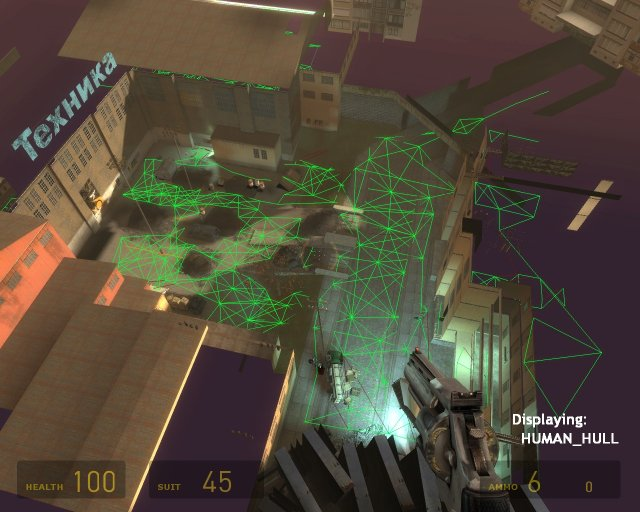
\includegraphics[width=\textwidth]{nodegraph} % https://developer.valvesoftware.com/wiki/Nodegraph
		\end{column}
		\begin{column}{0.58\textwidth}
			\begin{itemize}
				\pause\item Manually place graph nodes in the world
				\pause\item Place them at key points, e.g.\ in doorways, around obstacles
				\pause\item Works, but...
					\begin{itemize}
						\pause\item More work for level designers
						\pause\item Requires lots of testing and tweaking to get natural-looking results
						\pause\item No good for dynamic environments
					\end{itemize}
			\end{itemize}
		\end{column}
	\end{columns}
\end{frame}

\begin{frame}{Navigation meshes}
	\begin{columns}
		\begin{column}{0.4\textwidth}
			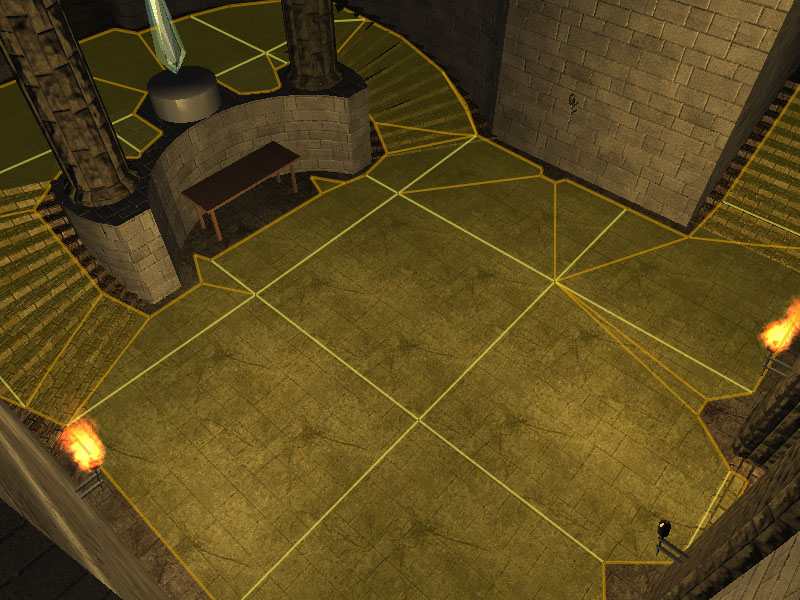
\includegraphics[width=\textwidth]{navmesh} % http://www.crystalspace3d.org/blog/leonardord?cat=53
		\end{column}
		\begin{column}{0.58\textwidth}
			\begin{itemize}
				\pause\item Automatically generate navigation graph from level geometry
				\pause\item Basic idea:
					\begin{itemize}
						\pause\item Filter level geometry to those polygons which are \textbf{passable}
							(i.e.\ floors, not walls/ceilings/obstacles)
						\pause\item Generate graph from polygons
					\end{itemize}
			\end{itemize}
		\end{column}
	\end{columns}
\end{frame}

\begin{frame}{Meshes to graphs}
	\begin{center}
		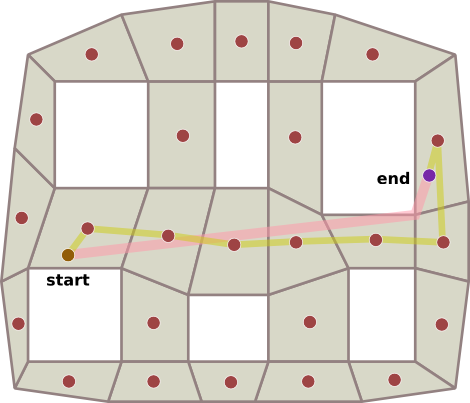
\includegraphics[width=0.6\textwidth]{polygon-navmesh-faces}
		% http://theory.stanford.edu/~amitp/GameProgramming/MapRepresentations.html
		
		Centres of polygons
	\end{center}
\end{frame}

\begin{frame}{Meshes to graphs}
	\begin{center}
		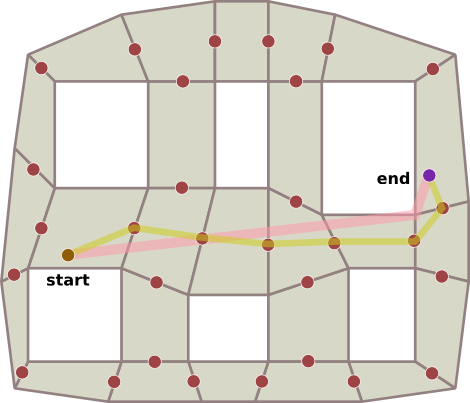
\includegraphics[width=0.6\textwidth]{polygon-navmesh-edges}
		% http://theory.stanford.edu/~amitp/GameProgramming/MapRepresentations.html
		
		Centres of edges
	\end{center}
\end{frame}

\begin{frame}{Meshes to graphs}
	\begin{center}
		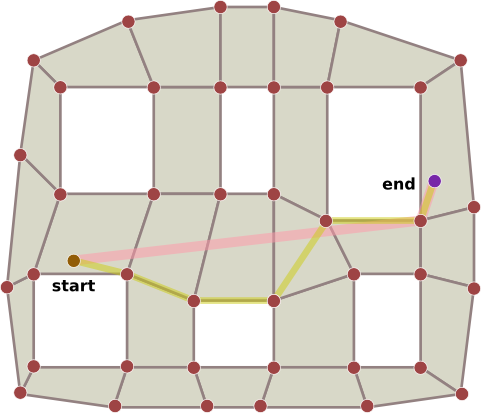
\includegraphics[width=0.6\textwidth]{polygon-navmesh-vertices}
		% http://theory.stanford.edu/~amitp/GameProgramming/MapRepresentations.html
		
		Vertices of polygons
	\end{center}
\end{frame}

\begin{frame}{Meshes to graphs}
	\begin{center}
		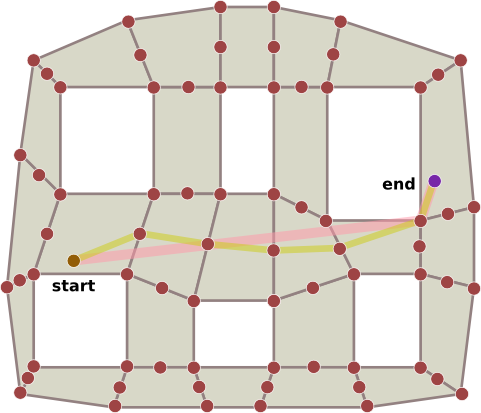
\includegraphics[width=0.6\textwidth]{polygon-navmesh-edges-and-vertices}
		% http://theory.stanford.edu/~amitp/GameProgramming/MapRepresentations.html
		
		Hybrid approach: edges and vertices
	\end{center}
\end{frame}

\begin{frame}{Following the path}
	\begin{itemize}
		\pause\item \textbf{Funnelling}: like string pulling but for navigation meshes
			\begin{itemize}
				\pause\item \url{http://digestingduck.blogspot.co.uk/2010/03/simple-stupid-funnel-algorithm.html}
				\item \url{http://jceipek.com/Olin-Coding-Tutorials/pathing.html}
			\end{itemize}
		\pause\item \textbf{Steering}: don't have your AI agent follow the path exactly, but
			instead try to stay close to it
		\pause\item \textbf{Dynamic environments}: may need to re-run pathfinder if environment changes
			(e.g.\ movable obstacles, destructible terrain)
	\end{itemize}
\end{frame}



\begin{frame}{Summary}
	\begin{itemize}
		\pause\item Pathfinding allows agents to navigate complex real or virtual environments
		\pause\item A* search (with appropriate heuristics) is an efficient algorithm for finding the optimal path from A to B
		\pause\item Navigation mesh generation allows A* to be applied to complex 3D game environments
	\end{itemize}
\end{frame}

\end{document}
